
In this example, we consider a classification problem where the goal is to
predict a target class, denoted by $Y$, from a set of observed nominal attributes $(\seqExp{A})$.
We assume that $Y$ may depend on an unknown subset of the attributes, rather than the full set.

This reflects a form of sparsity in the relationship between the class and the attributes, where irrelevant
features are ignored in the true generative model.

We can use the fused multinomial model of Example~\ref{ex:fused-multinomial} to capture this relationship.
As an example, assume that $Y$ depends only on $A_2$, $A_5$.
Then, we define the labeling function $f$ as follows:
\[
    f(\seqExp{A}, Y) = (A_2, A_5, Y) \cdot
\]
In a fused multinomial model with this labeling function, $Y$ will be conditionally independent
from other attributes, given $A_2, A_5$.
Additionally, $P(\seqExp{A} \mid A_2, A_5)$ will be uniform.

For every possible subset of attributes a distinct fused multinomial model of this form is needed.
Each model corresponds to a set of plausible distributions.
Definition~\ref{def:center-of-H} provides a way to define a central distribution for situations like this one.

By Theorem~\ref{th:lambda-centrality} we know that this central distribution would be a weighted average of
the central distributions of individual fused multinomial models.
Since we have a finite number of models, these weights are uniform:
\[
    C_{\setQQ}(S_n) \propto \sum_i C_{f_i}(S_n) \cdot
\]

To establish this, observe that we can construct a consistent estimator for the model indicator $I$ by checking
for the equality of different outcomes.
Specifically, the estimator identifies outcomes with equal frequency in the data and returns the indicator for
the model that supports this equality.

As shown in Equation~\ref{eq:bayes-action}, the optimal Bayesian decision rule depends on the chosen loss function.
In this example, we adopt the zero-one loss, which leads to predicting the label with the highest conditional
probability.
These probabilities are computed using the central distribution we previously derived.

To see how this approach works in practice, we carried out a synthetic experiment with the following setup.
We considered binary attributes and generated each attribute independently with equal probability for 0 and 1.
The class label was defined as a deterministic function of a fixed subset of 3 out of 12 total attributes, as
shown in Table~\ref{tab:functions}.
The same subset of relevant attributes and labeling function were used across all trials.

\begin{table}[htbp]
    \centering
    \caption{Mappings of 3-bit inputs under functions $f_1$ and $f_2$}
    \begin{tabular}{ccc}
        \toprule
        Input (bits) & $f_1$(Input) & $f_2$(Input) \\
        \midrule
        000          & a            & A            \\
        001          & b            & B            \\
        010          & c            & A            \\
        011          & d            & C            \\
        100          & e            & D            \\
        101          & f            & D            \\
        110          & g            & D            \\
        111          & h            & E            \\
        \bottomrule
    \end{tabular}\label{tab:functions}
\end{table}

For each experiment, we generated a training set of size 20 and a test set of size 60.
A larger test set was used to reduce variability in performance estimates, taking advantage of the synthetic
nature of the data.
To assess robustness to irrelevant features, we progressively removed one attribute at a time from the full set
of 12, starting with irrelevant ones and stopping just before removing any of the three relevant attributes.

At each step, we trained and tested two versions of the central distribution: one assuming a deterministic label
function (CD-Det) and one allowing for a conditional (non-deterministic) label distribution (CD-Prob).
Both versions are constructed by aggregating over $2^{12}$ fused multinomial models, corresponding to all subsets of
the 12 attributes.
As a baseline, we also trained a decision tree classifier (DTree).
All methods were trained on the same training data and evaluated on the same test data.
Each configuration was repeated for 100 independent trials, and we reported the average accuracy (correct
predictions divided by total test instances) over these trials.

\begin{figure}[htbp]
    \centering
    \caption{Accuracy vs. Number of Attributes (Function $f_1$, 20 train samples)}
    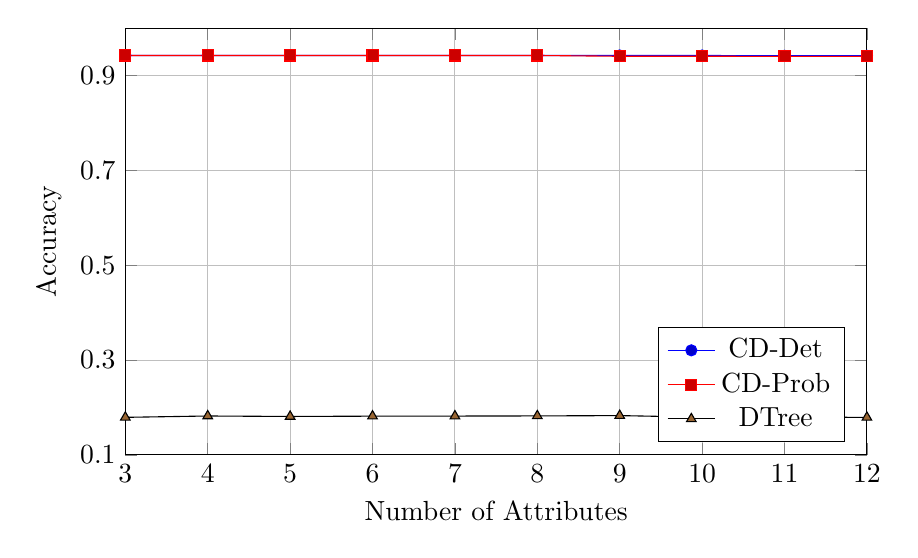
\begin{tikzpicture}
        \begin{axis}[
            width=11cm,
            height=7cm,
            xlabel={Number of Attributes},
            ylabel={Accuracy},
            xmin=3, xmax=12,
            ymin=0.1, ymax=1.0,
            xtick={3,4,5,6,7,8,9,10,11,12},
            ytick={0.1,0.3,0.5,0.7,0.9},
            legend pos=south east,
            grid=major,
            mark options={solid}
        ]

            \addplot+[mark=*, blue] coordinates {
                (3, 0.9425) (4, 0.9425) (5, 0.9425) (6, 0.9425) (7, 0.9425) (8, 0.9425) (9, 0.9425) (10, 0.9425) (11, 0.941833) (12, 0.941833)
            };
            \addlegendentry{CD-Det}

            \addplot+[mark=square*, red] coordinates {
                (3, 0.9425) (4, 0.9425) (5, 0.9425) (6, 0.9425) (7, 0.9425) (8, 0.9425) (9, 0.940833) (10, 0.940833) (11, 0.940667) (12, 0.940667)
            };
            \addlegendentry{CD-Prob}

            \addplot+[mark=triangle*, black] coordinates {
                (3, 0.179167) (4, 0.182) (5, 0.181) (6, 0.181667) (7, 0.181833) (8, 0.182167) (9, 0.182833) (10, 0.1795) (11, 0.18) (12, 0.179)
            };
            \addlegendentry{DTree}

        \end{axis}
    \end{tikzpicture}\label{fig:f1-results}
\end{figure}

\begin{figure}[htbp]
    \centering
    \caption{Accuracy vs. Number of Attributes (Function $f_2$, 20 train samples)}
    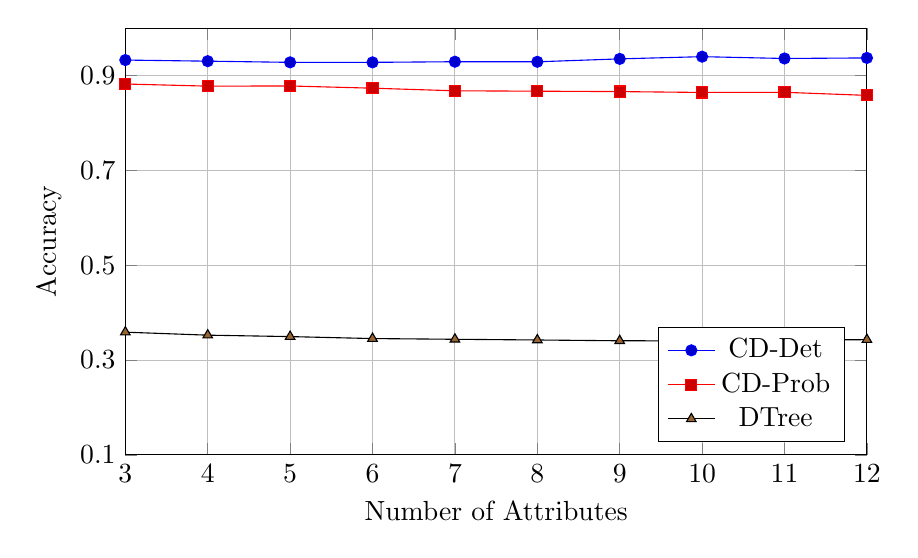
\begin{tikzpicture}
        \begin{axis}[
            width=11cm,
            height=7cm,
            xlabel={Number of Attributes},
            ylabel={Accuracy},
            xmin=3, xmax=12,
            ymin=0.1, ymax=1.0,
            xtick={3,4,5,6,7,8,9,10,11,12},
            ytick={0.1,0.3,0.5,0.7,0.9},
            legend pos=south east,
            grid=major,
            mark options={solid}
        ]

            \addplot+[mark=*, blue] coordinates {
                (3, 0.932833) (4, 0.9305) (5, 0.928) (6, 0.928) (7, 0.929333) (8, 0.929167) (9, 0.935333) (10, 0.94) (11, 0.936167) (12, 0.937333)
            };
            \addlegendentry{CD-Det}

            \addplot+[mark=square*, red] coordinates {
                (3, 0.882333) (4, 0.877833) (5, 0.878167) (6, 0.8735) (7, 0.868) (8, 0.867167) (9, 0.866333) (10, 0.8645) (11, 0.864833) (12, 0.858333)
            };
            \addlegendentry{CD-Prob}

            \addplot+[mark=triangle*, black] coordinates {
                (3, 0.358833) (4, 0.3525) (5, 0.3495) (6, 0.345333) (7, 0.343833) (8, 0.342333) (9, 0.340667) (10, 0.3405) (11, 0.342333) (12, 0.343)
            };
            \addlegendentry{DTree}

        \end{axis}
    \end{tikzpicture}\label{fig:f2-results}
\end{figure}

The results, shown in Figures~\ref{fig:f1-results} and~\ref{fig:f2-results}, reveal notable differences in
performance depending on the underlying class assignment function.
For function $f_1$, both deterministic and probabilistic methods achieve high accuracy, with the deterministic
version of the central distribution slightly outperforming the other.
In contrast, function $f_2$ is more difficult to predict, leading to a clearer separation in performance between the
two methods.
This difficulty primarily arises from strong non-deterministic dependencies between subsets of input bits and the
assigned label.
For instance, when the first input bit of $f_2$ is 1, the label is often D, creating a misleading
probabilistic association.
In this case, the deterministic central distribution remains the most accurate overall, while the probabilistic
version shows reduced performance due to misleading patterns.

\begin{figure}[htbp]
    \centering
    \caption{Accuracy vs. Number of Attributes (Function $f_2$, 10 train samples)}
    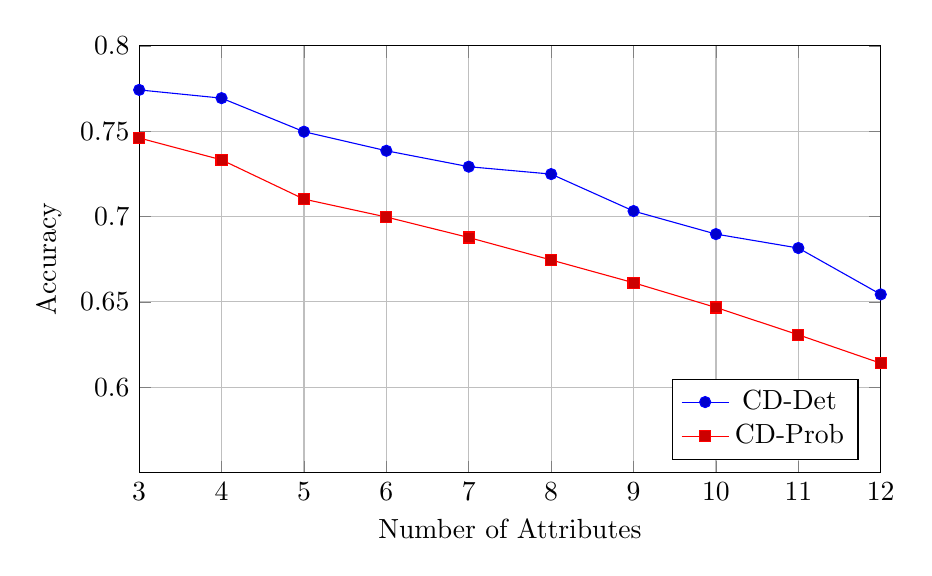
\begin{tikzpicture}
        \begin{axis}[
            width=11cm,
            height=7cm,
            xlabel={Number of Attributes},
            ylabel={Accuracy},
            xmin=3, xmax=12,
            ymin=0.55, ymax=0.8,
            xtick={3,4,5,6,7,8,9,10,11,12},
            ytick={0.6,0.65,0.7,0.75,0.8},
            legend pos=south east,
            grid=major,
            mark options={solid}
        ]

            \addplot+[mark=*, blue] coordinates {
                (3, 0.774167) (4, 0.769333) (5, 0.749667) (6, 0.7385) (7, 0.729167) (8, 0.724833) (9, 0.703167) (10, 0.689667) (11, 0.6815) (12, 0.654333)
            };
            \addlegendentry{CD-Det}

            \addplot+[mark=square*, red] coordinates {
                (3, 0.746) (4, 0.733167) (5, 0.710167) (6, 0.699667) (7, 0.687667) (8, 0.6745) (9, 0.661167) (10, 0.646667) (11, 0.630667) (12, 0.614)
            };
            \addlegendentry{CD-Prob}

        \end{axis}
    \end{tikzpicture}\label{fig:f2-10samples-results}
\end{figure}

While removing irrelevant attributes generally led to slight improvements in accuracy, the effect was not
substantial in our primary experiments with 20 training samples.
However, we observed that the benefit of attribute removal becomes more noticeable when the training set is
smaller.
In particular, additional experiments with 10 training samples showed a clearer performance gain as
irrelevant features were removed, indicating that the impact of irrelevant attributes is more pronounced in
low-data regimes (see Figure~\ref{fig:f2-10samples-results})

